% Options for packages loaded elsewhere
\PassOptionsToPackage{unicode}{hyperref}
\PassOptionsToPackage{hyphens}{url}
%
\documentclass[
  man,floatsintext]{apa6}
\usepackage{amsmath,amssymb}
\usepackage{iftex}
\ifPDFTeX
  \usepackage[T1]{fontenc}
  \usepackage[utf8]{inputenc}
  \usepackage{textcomp} % provide euro and other symbols
\else % if luatex or xetex
  \usepackage{unicode-math} % this also loads fontspec
  \defaultfontfeatures{Scale=MatchLowercase}
  \defaultfontfeatures[\rmfamily]{Ligatures=TeX,Scale=1}
\fi
\usepackage{lmodern}
\ifPDFTeX\else
  % xetex/luatex font selection
\fi
% Use upquote if available, for straight quotes in verbatim environments
\IfFileExists{upquote.sty}{\usepackage{upquote}}{}
\IfFileExists{microtype.sty}{% use microtype if available
  \usepackage[]{microtype}
  \UseMicrotypeSet[protrusion]{basicmath} % disable protrusion for tt fonts
}{}
\makeatletter
\@ifundefined{KOMAClassName}{% if non-KOMA class
  \IfFileExists{parskip.sty}{%
    \usepackage{parskip}
  }{% else
    \setlength{\parindent}{0pt}
    \setlength{\parskip}{6pt plus 2pt minus 1pt}}
}{% if KOMA class
  \KOMAoptions{parskip=half}}
\makeatother
\usepackage{xcolor}
\usepackage{graphicx}
\makeatletter
\def\maxwidth{\ifdim\Gin@nat@width>\linewidth\linewidth\else\Gin@nat@width\fi}
\def\maxheight{\ifdim\Gin@nat@height>\textheight\textheight\else\Gin@nat@height\fi}
\makeatother
% Scale images if necessary, so that they will not overflow the page
% margins by default, and it is still possible to overwrite the defaults
% using explicit options in \includegraphics[width, height, ...]{}
\setkeys{Gin}{width=\maxwidth,height=\maxheight,keepaspectratio}
% Set default figure placement to htbp
\makeatletter
\def\fps@figure{htbp}
\makeatother
\setlength{\emergencystretch}{3em} % prevent overfull lines
\providecommand{\tightlist}{%
  \setlength{\itemsep}{0pt}\setlength{\parskip}{0pt}}
\setcounter{secnumdepth}{-\maxdimen} % remove section numbering
% Make \paragraph and \subparagraph free-standing
\makeatletter
\ifx\paragraph\undefined\else
  \let\oldparagraph\paragraph
  \renewcommand{\paragraph}{
    \@ifstar
      \xxxParagraphStar
      \xxxParagraphNoStar
  }
  \newcommand{\xxxParagraphStar}[1]{\oldparagraph*{#1}\mbox{}}
  \newcommand{\xxxParagraphNoStar}[1]{\oldparagraph{#1}\mbox{}}
\fi
\ifx\subparagraph\undefined\else
  \let\oldsubparagraph\subparagraph
  \renewcommand{\subparagraph}{
    \@ifstar
      \xxxSubParagraphStar
      \xxxSubParagraphNoStar
  }
  \newcommand{\xxxSubParagraphStar}[1]{\oldsubparagraph*{#1}\mbox{}}
  \newcommand{\xxxSubParagraphNoStar}[1]{\oldsubparagraph{#1}\mbox{}}
\fi
\makeatother
% definitions for citeproc citations
\NewDocumentCommand\citeproctext{}{}
\NewDocumentCommand\citeproc{mm}{%
  \begingroup\def\citeproctext{#2}\cite{#1}\endgroup}
\makeatletter
 % allow citations to break across lines
 \let\@cite@ofmt\@firstofone
 % avoid brackets around text for \cite:
 \def\@biblabel#1{}
 \def\@cite#1#2{{#1\if@tempswa , #2\fi}}
\makeatother
\newlength{\cslhangindent}
\setlength{\cslhangindent}{1.5em}
\newlength{\csllabelwidth}
\setlength{\csllabelwidth}{3em}
\newenvironment{CSLReferences}[2] % #1 hanging-indent, #2 entry-spacing
 {\begin{list}{}{%
  \setlength{\itemindent}{0pt}
  \setlength{\leftmargin}{0pt}
  \setlength{\parsep}{0pt}
  % turn on hanging indent if param 1 is 1
  \ifodd #1
   \setlength{\leftmargin}{\cslhangindent}
   \setlength{\itemindent}{-1\cslhangindent}
  \fi
  % set entry spacing
  \setlength{\itemsep}{#2\baselineskip}}}
 {\end{list}}
\usepackage{calc}
\newcommand{\CSLBlock}[1]{\hfill\break\parbox[t]{\linewidth}{\strut\ignorespaces#1\strut}}
\newcommand{\CSLLeftMargin}[1]{\parbox[t]{\csllabelwidth}{\strut#1\strut}}
\newcommand{\CSLRightInline}[1]{\parbox[t]{\linewidth - \csllabelwidth}{\strut#1\strut}}
\newcommand{\CSLIndent}[1]{\hspace{\cslhangindent}#1}
\ifLuaTeX
\usepackage[bidi=basic]{babel}
\else
\usepackage[bidi=default]{babel}
\fi
\babelprovide[main,import]{english}
% get rid of language-specific shorthands (see #6817):
\let\LanguageShortHands\languageshorthands
\def\languageshorthands#1{}
% Manuscript styling
\usepackage{upgreek}
\captionsetup{font=singlespacing,justification=justified}

% Table formatting
\usepackage{longtable}
\usepackage{lscape}
% \usepackage[counterclockwise]{rotating}   % Landscape page setup for large tables
\usepackage{multirow}		% Table styling
\usepackage{tabularx}		% Control Column width
\usepackage[flushleft]{threeparttable}	% Allows for three part tables with a specified notes section
\usepackage{threeparttablex}            % Lets threeparttable work with longtable

% Create new environments so endfloat can handle them
% \newenvironment{ltable}
%   {\begin{landscape}\centering\begin{threeparttable}}
%   {\end{threeparttable}\end{landscape}}
\newenvironment{lltable}{\begin{landscape}\centering\begin{ThreePartTable}}{\end{ThreePartTable}\end{landscape}}

% Enables adjusting longtable caption width to table width
% Solution found at http://golatex.de/longtable-mit-caption-so-breit-wie-die-tabelle-t15767.html
\makeatletter
\newcommand\LastLTentrywidth{1em}
\newlength\longtablewidth
\setlength{\longtablewidth}{1in}
\newcommand{\getlongtablewidth}{\begingroup \ifcsname LT@\roman{LT@tables}\endcsname \global\longtablewidth=0pt \renewcommand{\LT@entry}[2]{\global\advance\longtablewidth by ##2\relax\gdef\LastLTentrywidth{##2}}\@nameuse{LT@\roman{LT@tables}} \fi \endgroup}

% \setlength{\parindent}{0.5in}
% \setlength{\parskip}{0pt plus 0pt minus 0pt}

% Overwrite redefinition of paragraph and subparagraph by the default LaTeX template
% See https://github.com/crsh/papaja/issues/292
\makeatletter
\renewcommand{\paragraph}{\@startsection{paragraph}{4}{\parindent}%
  {0\baselineskip \@plus 0.2ex \@minus 0.2ex}%
  {-1em}%
  {\normalfont\normalsize\bfseries\itshape\typesectitle}}

\renewcommand{\subparagraph}[1]{\@startsection{subparagraph}{5}{1em}%
  {0\baselineskip \@plus 0.2ex \@minus 0.2ex}%
  {-\z@\relax}%
  {\normalfont\normalsize\itshape\hspace{\parindent}{#1}\textit{\addperi}}{\relax}}
\makeatother

\makeatletter
\usepackage{etoolbox}
\patchcmd{\maketitle}
  {\section{\normalfont\normalsize\abstractname}}
  {\section*{\normalfont\normalsize\abstractname}}
  {}{\typeout{Failed to patch abstract.}}
\patchcmd{\maketitle}
  {\section{\protect\normalfont{\@title}}}
  {\section*{\protect\normalfont{\@title}}}
  {}{\typeout{Failed to patch title.}}
\makeatother

\usepackage{xpatch}
\makeatletter
\xapptocmd\appendix
  {\xapptocmd\section
    {\addcontentsline{toc}{section}{\appendixname\ifoneappendix\else~\theappendix\fi: #1}}
    {}{\InnerPatchFailed}%
  }
{}{\PatchFailed}
\makeatother
\keywords{child development, egocentric video, audio dataset, multimodal learning, computer vision, developmental psychology}
\usepackage{csquotes}
\ifLuaTeX
  \usepackage{selnolig}  % disable illegal ligatures
\fi
\usepackage{bookmark}
\IfFileExists{xurl.sty}{\usepackage{xurl}}{} % add URL line breaks if available
\urlstyle{same}
\hypersetup{
  pdftitle={ChildLens: An Egocentric Video Dataset for Activity Analysis in Children},
  pdfauthor={Nele-Pauline Suffo1, Pierre-Etienne Martin2, Daniel Haun2, \& Manuel Bohn1, 2},
  pdflang={en-EN},
  pdfkeywords={child development, egocentric video, audio dataset, multimodal learning, computer vision, developmental psychology},
  hidelinks,
  pdfcreator={LaTeX via pandoc}}

\title{ChildLens: An Egocentric Video Dataset for Activity Analysis in Children}
\author{Nele-Pauline Suffo\textsuperscript{1}, Pierre-Etienne Martin\textsuperscript{2}, Daniel Haun\textsuperscript{2}, \& Manuel Bohn\textsuperscript{1, 2}}
\date{}


\shorttitle{ChildLens Dataset}

\authornote{

The authors made the following contributions. Nele-Pauline Suffo: Conceptualization, Writing - Original Draft Preparation, Writing - Review \& Editing; Manuel Bohn: Writing - Review \& Editing, Supervision.

Correspondence concerning this article should be addressed to Nele-Pauline Suffo, Universitätsallee 1, 21335 Lüneburg. E-mail: \href{mailto:nele.suffo@leuphana.de}{\nolinkurl{nele.suffo@leuphana.de}}

}

\affiliation{\vspace{0.5cm}\textsuperscript{1} Institute of Psychology in Education, Leuphana University Lüneburg\\\textsuperscript{2} Max Planck Institute for Evolutionary Anthropology}

\abstract{%
We present ChildLens, a novel egocentric video and audio dataset of children aged 3--5 years, featuring detailed activity labels. Spanning 106 hours of recordings, the dataset includes five location classes and 14 activity classes, covering audio-only, video-only, and multimodal activities. Captured through a vest equipped with an embedded camera, ChildLens provides a rich resource for analyzing children's daily interactions and behaviors. We provide an overview of the dataset, the collection process, and the labeling strategy. Additionally, we present benchmark performance of two state-of-the-art models on the dataset: the Boundary-Matching Network for Temporal Activity Localization and the Voice-Type Classifier for detecting and classifying speech in audio. Finally, we analyze the dataset specifications and their influence on model performance. The ChildLens dataset will be made available for research purposes, providing rich data to advance computer vision and audio analysis techniques while offering new insights into developmental psychology.
}



\begin{document}
\maketitle

\section{Introduction}\label{introduction}

In developmental psychology, everyday experiences are crucial for shaping children's development (Carpendale \& Lewis, 2020; Heyes, 2018; Piaget, 1964; Rogoff, Dahl, \& Callanan, 2018; Smith, Jayaraman, Clerkin, \& Yu, 2018; Tomasello, 2009; Vygotsky, 1978). Fundamental theories, such as Piaget's Learning Theory of Cognitive Development (Piaget, 1964), have long recognized the role of everyday interactions in helping children actively construct knowledge, whereas Vygotsky's Sociocultural Theory (Vygotsky, 1978) emphasized how social interactions help transform everyday sensory experiences into structured understanding. Building on these foundational insights, more recent studies have further explored how everyday experiences shape cognitive and social development. For instance, Spangler (Spangler, 1989) showed that toddlers' daily interactions shape their mental and emotional dispositions, predicting later developmental outcomes. Similarly, Tomasello's Cultural Learning Theory (Tomasello, 2009) pointed out how everyday social interactions, particularly those involving shared intentionality, foster uniquely human cognitive abilities by enabling children to understand others' intentions and perspectives. Further expanding on this, Heyes's work on the Cultural Evolution of Thinking (Heyes, 2018) highlighted the importance of experiences like imitation and informal social learning in developing cognitive capacities. Debarbaro et al. (De Barbaro \& Fausey, 2022) summarized various studies, emphasizing the need to analyze infants' dynamic, diverse experiences captured through everyday activity sensors, and stressed the significance of long-term analysis to understand developmental patterns and variability. Despite this growing body of work, direct research connecting the diversity of children's daily experiences to broader developmental trajectories remains limited. Whereas many studies focus on specific domains such as language or social cognition, there remains a need for more comprehensive investigations into how diverse daily experiences shape developmental trajectories.

In the context of children's developmental trajectories, research has focused on areas like language acquisition, theory of mind, and social cognition, utilizing a range of methods and data sources. For instance, Donnelly et al. (Donnelly \& Kidd, 2021) used audio-only data to explore the relationship between conversational turn-taking and vocabulary growth in children, whereas Roy et al. (Roy, Frank, DeCamp, Miller, \& Roy, 2015) examined how words used in specific contexts are learned more easily, emphasizing the importance of multimodal contexts. In contrast, Rowe (Rowe \& Goldin-Meadow, 2009) leveraged video data to investigate how gestures at 14 months predict vocabulary development in children from different socioeconomic backgrounds. Ruffman et al. (Ruffman et al., 2023) used head-mounted video cameras to study how repeated behaviors in everyday life correlate with the acquisition of mental state vocabulary, supporting the minimalist view of theory of mind development. Bergelson (Bergelson et al., 2023), on the other hand, used large-scale audio data to explore the impact of adult speech on children's language production across diverse cultural contexts. These studies demonstrate the value of both audio and video data in understanding children's development, yet they highlight the need for datasets that capture the full diversity of children's everyday experiences.

A significant challenge in this field is the extensive amount of data needed to comprehensively study children's daily lives. Traditional methods, such as manual annotation, are time-consuming and impractical for large-scale datasets. To address this, computational models offer scalable solutions for analyzing social interactions and behaviors. For instance, OpenPose (Cao, Hidalgo, Simon, Wei, \& Sheikh, 2018) allows the tracking of human body, face, and hand poses, providing insights into gestures and engagement. YOLOv8 (Redmon, Divvala, Girshick, \& Farhadi, 2015) offers efficient object detection for analyzing children's interactions with their environment, whereas models like I3D (Carreira \& Zisserman, 2017) provide an automataed solution for classifying activities in video data. For audio, Wave2Vec 2.0 (Baevski, Zhou, Mohamed, \& Auli, 2020) provides robust speech-to-text and speech representation capabilities, enabling the study of conversational dynamics. Together, these models facilitate the efficient analysis of multimodal data, but their improvement and development depend on the availability of diverse, high-quality datasets. A notable example of such a dataset is ImageNet (Russakovsky et al., 2014), which has been crucial in advancing computer vision models. Similarly, expanding publicly available datasets in developmental psychology could accelerate progress in studying children's everyday experiences.

Several publicly available datasets have made valuable contributions to our understanding of children's social and communicative behavior. For example, the SAYCam dataset (Sullivan, Mei, Perfors, Wojcik, \& Frank, 2021) provides audio-video recordings from infants (6--32 months) who wore head-mounted cameras over two years, capturing naturalistic speech and behaviors. Similarly, the DAMI-P2C dataset (Chen, Alghowinem, Jang, Breazeal, \& Park, 2023) includes audio and video recordings of parent-child interactions during story reading, with annotations for body movements in a controlled environment. The MMDB dataset (Rehg et al., 2013) offers multimodal data (audio, video, physiological) of children (15--30 months) engaged in semi-structured play interactions, recorded in a lab. Another example is the UpStory dataset (Fraile et al., 2024), which features audio and video of primary school children (8-10 years) in dyadic storytelling interactions, also recorded in a lab setting. Additionally, the BabyView dataset (Long et al., 2024) provides high-resolution, egocentric video of children aged 6 months to 5 years, recorded at home and in preschool environments, with annotations for speech transcription and pose estimation. Whereas these datasets vary in age, setting, and target behaviors, they collectively highlight the need for more naturalistic, at-home datasets that can capture the full range of children's daily activities.

To address this gap, we introduce the publicly available ChildLens dataset, which focuses on activity annotations for children aged 3--5 years and captures their naturalistic experiences at home. The dataset consists of 106 hours of video and audio recordings collected from 61 children wearing camera-equipped vests. It includes detailed activity annotations for five location classes and 14 activity classes, categorizing activities based on whether the child is interacting alone or with others. These annotations, labeled with start and end times, provide a granular view of children's everyday behaviors, crucial for understanding their developmental trajectories. Designed to support research in developmental psychology and computer vision, the ChildLens dataset offers a rich resource for advancing multimodal learning and studying the full spectrum of children's daily activities.

\section{Dataset Overview}\label{dataset-overview}

\paragraph{Activity Classes}\label{activity-classes}

The ChildLens dataset includes 14 activity classes and 5 location classes. The activity classes are categorized based on the child's interactions within the video and can be divided into \emph{person-only} activities (e.g.~``child talking'', ``other person talking''), and \emph{person-object} activities (e.g.~``drawing'', ``playing with object''). A brief description of each class can be found in the appendix. These activities are further categorized into \emph{audio-based}, \emph{visual-based}, and \emph{multimodal} activities, as presented in Figure \ref{fig:camera-superannotate-activity-classes}. Below is an overview of the different activity types:

\begin{itemize}
\tightlist
\item
  \textbf{Audio-based activities}: \emph{child talking}, \emph{other person talking}, \emph{overheard speech}, \emph{singing / humming}, \emph{listening to music / audiobook}
\item
  \textbf{Visual-based activities}: \emph{watching something}, \emph{drawing}, \emph{crafting things}, \emph{dancing}
\item
  \textbf{Multimodal activities}: \emph{playing with object}, \emph{playing without object}, \emph{making music}, \emph{pretend play}, \emph{reading book}
\end{itemize}

The location classes describe the current location of the child in the video and include \emph{livingroom}, \emph{playroom}, \emph{bathroom}, \emph{hallway}, and \emph{other}.

\begin{figure}

{\centering 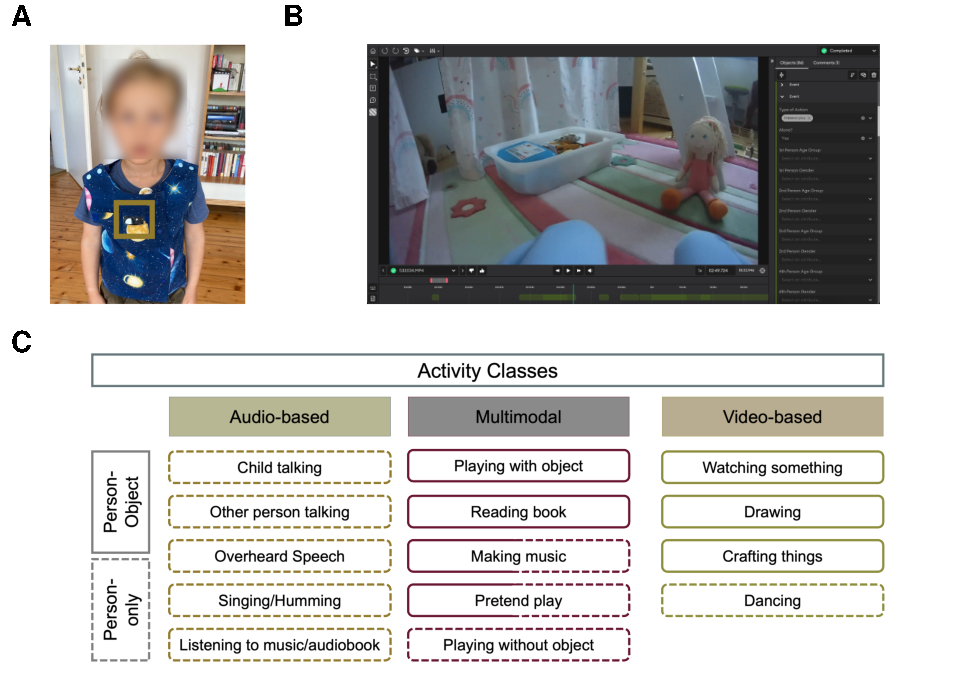
\includegraphics{ChildLens_paper_files/figure-latex/camera-superannotate-activity-classes-1} 

}

\caption{\textbf{A} – Vest with the embedded camera worn by the children, \textbf{B} – SuperAnnotate platform utilized for video annotation, \textbf{C} – Activity classes in the ChildLens dataset.}\label{fig:camera-superannotate-activity-classes}
\end{figure}

\paragraph{Statistics}\label{statistics}

The ChildLens dataset comprises of 343 video files with a total of 106.10 hours recorded by 61 children aged 3 to 5 years (M=4.52, SD=0.92). This includes 107 videos from children aged 3, 122 videos from children aged 4, and 114 videos from children aged 5. The video duration per child varies between 4.03 and 303.42 minutes (M=104.37, SD=51.65). A detailed distribution of the video duration per child is shown in figure \ref{fig:minutes-per-child}.

This diverse dataset includes a varying number of instances across the 14 activity classes, with each class containing between 2 and 319 instances per class. The duration of each instance varies by activity. For instance, audio-based activities like ``child talking'' may last only a few seconds, while activities like ``reading a book'' can span several minutes. The table with the total number of instances and summed duration for all activity classes is available in the appendix.

\begin{figure}
\centering
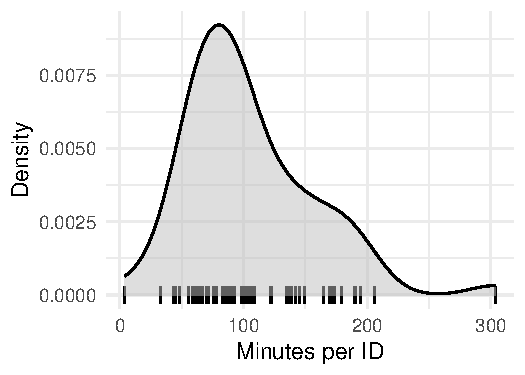
\includegraphics{ChildLens_paper_files/figure-latex/minutes-per-child-1.pdf}
\caption{\label{fig:minutes-per-child}Video recording duration (in minutes) per child ID.}
\end{figure}

\paragraph{Data Access}\label{data-access}

The ChildLens dataset will be made available for research purposes, providing a rich resource for studying children's daily activities and interactions. The dataset includes video and audio recordings, along with activity labels. Due to the sensitive nature of the data---recordings of children in their homes---access will be restricted.

As the annotation process is still ongoing, the dataset will be updated regularly. A brief project overview and the latest dataset version can be found \href{https://www.eva.mpg.de/comparative-cultural-psychology/technical-development/childlens/}{here} Researchers can submit requests for access through the , which will be carefully reviewed to ensure proper handling and compliance with privacy standards. Please contact person to request access to the dataset.

\paragraph{Exhaustive multi-label annotations}\label{exhaustive-multi-label-annotations}

The dataset provides detailed annotations for each video file. These annotations specify the child's current location within the video, the start and end times of each activity, the activity class, and whether the child is engaged alone or with somebody else. For every person involved in the activity, we capture age and gender. If multiple activities occur simultaneously in a video, each activity is individually labeled. For example, if a segment shows a child ``reading a book'' while also ``talking,'' two separate annotations are created: one for ``reading a book'' and another for ``child talking.'' This exhaustive labeling strategy ensures that each activity is accurately represented in the dataset.

\section{Dataset Generation}\label{dataset-generation}

This section outlines the steps taken to create the ChildLens dataset. We provide detailed information on the video collection process, the labeling strategy employed, and the generation of activity labels.

\subsection{Step 1: Collection of Egocentric Videos}\label{step-1-collection-of-egocentric-videos}

The ChildLens dataset consists of egocentric videos recorded by children aged 3 to 5 years over a period of 12 months. A total of 61 children from families living in a mid-sized city in Germany, participated in the study. The videos were captured at home using a camera embedded in a vest worn by the children, as shown in figure \ref{fig:camera-superannotate-activity-classes}. This setup allowed the children to move freely throughout their homes while recording their activities. The camera, a \emph{PatrolEyes WiFi HD Infrared Police Body Camera}, was equipped with a 140-degree wide-angle lens and captured everything within the child's field of view with a resolution of 1920x1080p at 30 fps. The camera also recorded audio, allowing us to capture the child's speech and other sounds in the environment. Additionally, the parents were handed a small checklist of activities to record, ensuring that a variety of activities were represented in the videos. The focus was on capturing everyday activities that children typically engage in. Parents were therefore asked to include the following elements in the recordings:

\begin{itemize}
\tightlist
\item
  Child spends time in different rooms and performs various activities in each room
\item
  Child is invited to read a book together with an adult
\item
  Child is invited to play with toys alone
\item
  Child is invited to play with toys with someone else (adult or child)
\item
  Child is invited to draw/craft something
\end{itemize}

\subsection{Step 2: Creation of Labeling Strategy}\label{step-2-creation-of-labeling-strategy}

To create a comprehensive labeling strategy for the ChildLens dataset, we first defined a list of activities that children typically engage in. This list was based on previous research on child development and the activities that children are known to participate in. We then developed a detailed catalog of activities that were likely to be captured in the videos and chose to make the activity classes more granular by distinguishing between activities like ``making music'' and ``singing/humming'' or ``drawing'' and ``crafting things''.

After an initial review of the videos, we decided to add another class ``overheard speech'' to capture situations in which the child is not directly involved in a conversation but can hear it. We also added ``pretend play'' as a separate class to capture situations in which the child is engaged in imaginative play. This approach allowed us to capture the diversity of activities that children engage in and create a comprehensive dataset for activity analysis.

\subsection{Step 3: Manual Labeling Process}\label{step-3-manual-labeling-process}

Before the actual annotation process, a setup meeting was held to introduce the annotators to the labeling strategy. To familiarize themselves with the task, the annotators were assigned 25 sample videos to practice and gain hands-on experience. These initial annotations were reviewed by the research team, and feedback was provided to refine the approach. A total of three feedback loops were conducted to ensure that the annotators follow the labeling strategy properly.

The videos were manually annotated by native German speakers who watched each video and labeled the activities present in the footage. Annotators marked the start and end points of each activity. For audio annotations, we implemented a 2-second rule for the categories `other person talking' and `child talking': if the break between two utterances was 2 seconds or less, it was considered a single event; breaks longer than 2 seconds split the activity into separate instances. The annotations were conducted using the SuperAnnotate platform, as shown in figure \ref{fig:camera-superannotate-activity-classes}, allowing for efficient annotation and review of the videos.

\section{Benchmark Performance}\label{benchmark-performance}

In this chapter, we present the results of applying two model architectures to the ChildLens dataset. While the dataset supports multimodal activity analysis, we focus on two specific tasks: temporal activity localization using video data and voice type classification using audio data. For temporal activity localization, we use the Boundary-Matching Network (BMN) model, a state-of-the-art approach in this domain, and train it from scratch on the unique activity classes in the ChildLens video data. For voice type classification, we apply the Voice Type Classifier (VTC) (Lavechin, Bousbib, Bredin, Dupoux, \& Cristia, 2020), also state-of-the-art, which was trained on similar data. Both models provide initial results and establish a benchmark for future research.

\subsection{Temporal Activity Localization}\label{temporal-activity-localization}

We employ the Boundary-Matching Network (BMN) (Lin, Liu, Li, Ding, \& Wen, 2019) for temporal activity localization on our dataset. BMN generates action proposals by predicting activity start and end boundaries and classifying these proposals into activity classes. The architecture consists of two main components: (1) a proposal generation network, which identifies candidate proposals, and (2) a proposal classification network, which classifies these proposals. The model prioritizes proposals with high recall and high temporal overlap with ground truth.
BMN performance is evaluated using Average Recall (AR) and Area Under the Curve (AUC) metrics. AR is computed at various Intersection over Union (IoU) thresholds and for different Average Numbers of Proposals (AN) as \href{mailto:AR@AN}{\nolinkurl{AR@AN}}, where AN ranges from 0 to 100. \href{mailto:AR@100}{\nolinkurl{AR@100}} reflects recall performance with 100 proposals per video, while AUC quantifies the trade-off between recall and number of generated proposal On the ActivityNet-1.3 test set, BMN achieves an \href{mailto:AR@100}{\nolinkurl{AR@100}} of 72.46 and an AUC of 64.47, demonstrating its effectiveness in activity localization.

\subsubsection{Data Preparation}\label{data-preparation}

The BMN implementation, including video preprocessing and model training, was conducted using the MMAction2 toolbox (Contributors, 2020). Data preparation involved several key steps, such as raw frame extraction and the generation of both RGB and optical flow features for each video. Before training the model, we analyzed the distribution of activity instances across the classes to assess the data's sufficiency for both training and testing. A detailed summary of the activity instances and their total durations can be found in the appendix.

Our analysis highlighted a significant class imbalance in the dataset, both in terms of instance count and the total duration of recordings. Given the primary goal of establishing initial benchmark results, no data augmentation methods were employed to mitigate this imbalance. Instead, the focus was placed on the more frequent activity classes, which also had the longest durations: ``Playing with Object'' (22.85 hours of recording), ``Drawing'' (6.24 hours of recording), and ``Reading a Book'' (5.48 hours of recording).

For feature extraction and model training optimization, the videos were divided into clips of 4000 frames each (correspond to approx. 2 minutes and 13 seconds). This resulted in a total of 1130 clips. However, only 995 clips had annotations, so we split these annotated clips into training, validation, and test subsets, using an 80-10-10 split. The training set was used for model optimization, the validation set guided hyperparameter tuning and overfitting prevention, and the test set was reserved for evaluating the model's generalization ability on unseen data.

\subsubsection{Implementation Details}\label{implementation-details}

The BMN model was trained from scratch on the ChildLens dataset to predict the start and end boundaries of activity classes in the videos. The model was implemented using MMAction2, an open-source toolbox for video understanding based on PyTorch (Contributors, 2020). Training took place on a Linux server with 48 cores and 187 GB of RAM. The Adam optimizer was used with a learning rate of 0.001 and a batch size of 4. To avoid overfitting, early stopping based on validation loss was applied during training.

\subsubsection{Evaluation}\label{evaluation}

The performance of the BMN model on the ChildLens dataset, compared to its evaluation on ActivityNet-1.3, is summarized in Table \ref{tab:bmn-results}, with \href{mailto:AR@100}{\nolinkurl{AR@100}} and AUC reported for both datasets. The results indicate that the BMN model generalizes well to new domains, such as children's everyday activities, despite the ChildLens dataset's focus on social and behavioral interactions in naturalistic settings. These benchmark results highlight the potential for integrating the ChildLens dataset with existing models like BMN. Automating the analysis of this dataset can streamline the study of children's activities and interactions, facilitating more efficient research in developmental psychology and related fields.

\begin{table}[tbp]

\begin{center}
\begin{threeparttable}

\caption{\label{tab:bmn-results}Comparison of BMN performance on the ActivityNet-1.3 dataset (used for model evaluation) and the ChildLens dataset, highlighting the Average Recall for 100 proposals (AR@100) and the Area Under the Curve (AUC).}

\begin{tabular}{lll}
\toprule
Dataset & \multicolumn{1}{c}{AR@100} & \multicolumn{1}{c}{AUC}\\
\midrule
ActivityNet-1.3 & 72.46 & 64.47\\
ChildLens & 77.43 & 69.21\\
\bottomrule
\end{tabular}

\end{threeparttable}
\end{center}

\end{table}

\subsection{Voice Type Classification}\label{voice-type-classification}

Voice Type Classification is the task of identifying audio utterances and assigning them to predefined classes: \texttt{Key\ Child\ (KCHI)}, \texttt{Other\ Child\ (CHI)}, \texttt{Male\ Speech\ (MAL)}, \texttt{Female\ Speech\ (FEM)}, and \texttt{Speech\ (SPEECH)} (Lavechin et al., 2020). The Voice Type Classifier model (VTC) is designed to perform this task efficiently. Its architecture is composed of a SincNet layer, two bi-directional LSTMs, and three feed-forward layers. The model takes a 2-second audio chunk as input and outputs a score between 0 and 1 for each class. The VTC was originally trained on 260 hours of child-centered audio recordings, which closely resembles our dataset in both structure and context.

Leveraging the capabilities of the open-source pyannote library for speaker diarization (Bredin, 2023; Plaquet \& Bredin, 2023), we evaluated the ChildLens dataset's quality through three distinct VTC training setups:

\begin{enumerate}
\def\labelenumi{\arabic{enumi}.}
\tightlist
\item
  \textbf{Direct Application}: Pretrained VTC model applied to ChildLens as-is.
\item
  \textbf{Fine-tuned:}: Pretrained VTC fine-tuned on ChildLens.
\item
  \textbf{Training from Scratch}: VTC trained solely on ChildLens.
\end{enumerate}

These setups test the dataset's annotation consistency and standalone value, with performance measured by the \(F_1\)-measure, which combines precision and recall using the following formula:
\[
F_1 = 2 \cdot \frac{\text{precision} \cdot \text{recall}}{\text{precision} + \text{recall}}
\]
where \(\text{precision} = \frac{\text{tp}}{\text{tp} + \text{fp}}\) and \(\text{recall} = \frac{\text{tp}}{\text{tp} + \text{fn}}\) with

\begin{itemize}
\tightlist
\item
  \(\text{tp}\) being the number of true positives,
\item
  \(\text{fp}\) being the number of false positives, and
\item
  \(\text{fn}\) being the number of false negatives.
\end{itemize}

Ranging from 0 to 1, \(F_1\)\textgreater{} 0.8 score is considered good and \(F_1\) \textgreater{} 0.9 as excellent.

\subsubsection{Data Preparation}\label{data-preparation-1}

We used the following mapping strategy to align our audio-based activity classes with the VTC's output classes:

\begin{itemize}
\tightlist
\item
  Child talking → \textbf{\texttt{Key\ Child}} \& \textbf{\texttt{Speech}}
\item
  Singing/Humming → \textbf{\texttt{Key\ Child}} \& \textbf{\texttt{Speech}}
\item
  Other person talking:

  \begin{itemize}
  \tightlist
  \item
    If \texttt{age\ =\ "Child"} → \textbf{\texttt{Other\ Child}} \& \textbf{\texttt{Speech}}
  \item
    If \texttt{age\ =\ "Adult"} \& \texttt{gender\ =\ "Female"} → \textbf{\texttt{Female\ Speech}} \& \textbf{\texttt{Speech}}
  \item
    If \texttt{age\ =\ "Adult"} \& \texttt{gender\ =\ "Male"} → \textbf{\texttt{Male\ Speech}} \& \textbf{\texttt{Speech}}
  \end{itemize}
\item
  Overheard Speech → \textbf{\texttt{Speech}}
\end{itemize}

``Listening to music/audiobook'' was excluded, as it's often background audio, lacks speaker age/gender details, and includes music irrelevant to VTC. ``Overheard Speech'', indicating speech not directed at the key child, was mapped to SPEECH due to missing age/gender annotations, potentially underestimating VTC performance (e.g., correct FEM predictions scored as SPEECH). In this context, we retain this mapping, as re-annotation would be time-consuming, and the class is designed for complex models, like NLP architectures, that can detect the speech recipient context effectively. Total durations for each VTC class are shown in Table \ref{tab:vtc-classes-statistics}.

\subsubsection{Implementation Details}\label{implementation-details-1}

We first applied te pretrained VTC model directly, using the available VTC implementation. We then fine-tuned the model on our ChildLens dataset for 200 epochs (12.86 hours) on the same Linux server as the BMN model. Finally, we trained the VTC model from scratch for 200 epochs (12.86 hours) using the ChildLens dataset to assess its standalone value

\begin{table}[tbp]

\begin{center}
\begin{threeparttable}

\caption{\label{tab:vtc-classes-statistics}Cumulative Duration (in minutes) of Utterances Categorized by Voice Type}

\begin{tabular}{llllll}
\toprule
 & \multicolumn{1}{c}{KCHI} & \multicolumn{1}{c}{CHI} & \multicolumn{1}{c}{MAL} & \multicolumn{1}{c}{FEM} & \multicolumn{1}{c}{SPEECH}\\
\midrule
Total Duration & 859.27 & 43.98 & 200.41 & 455.90 & 2361.87\\
\bottomrule
\end{tabular}

\end{threeparttable}
\end{center}

\end{table}

\subsubsection{Evaluation}\label{evaluation-1}

Table \ref{tab:vtc-results} shows \(F_1\)-scores for three VTC setups on the ChildLens dataset: the original model \(VTC_{og}\), fine-tuned model \(VTC_{ft}\), and model trained from scratch \(VTC_{cl}\), compared to the benchmark dataset. \(VTC_{og}\) scores 41.70, slightly below the benchmark, with best performance on \texttt{KCHI} (62.80) and worst on \texttt{CHI} (5.30). Fine-tuning \(VTC_{ft}\) training from scratch \(VTC_{cl}\) achieve 54.50 and 53.20, respectively, showing significant improvement. The low \texttt{CHI} scores are primarily due to frequent misclassifications as \texttt{KCHI}. This likely results from the vocal similarity between the key child and other children in the ChildLens dataset. In many cases, distinguishing between them may rely more on acoustic cues like proximity to the microphone than on vocal characteristics. In contrast, the original VTC dataset includes audio from infants and toddlers, where the distinction between the key child (often babbling or younger) and other speakers is more pronounced, making classification tasks easier. Importantly, these scores are expected to improve as more annotated data becomes available, since annotation is still ongoing. Figure \ref{fig:vtc-evaluations} visualizes how model predictions compare to the ground truth annotations for the \(VTC_{ft}\) model.

\begin{table}[tbp]

\begin{center}
\begin{threeparttable}

\caption{\label{tab:vtc-results}Comparison of Voice Type Classifier (VTC) performance on the ACLEW-Random dataset and the three setups utilizing the ChildLens dataset. The evaluation metrics are reported for the original VTC model (VTC-OG), the VTC fine-tuned on ChildLens (VTC-FT) and the VTC trained from scratch on ChildLens (VTC-CL). The table reports the F1 score per class and the average F1 score (AVG).
}

\begin{tabular}{llllllll}
\toprule
Dataset & \multicolumn{1}{c}{Architecture} & \multicolumn{1}{c}{KCHI} & \multicolumn{1}{c}{CHI} & \multicolumn{1}{c}{MAL} & \multicolumn{1}{c}{FEM} & \multicolumn{1}{c}{SPEECH} & \multicolumn{1}{c}{AVG}\\
\midrule
ACLEW-Random & VTC-OG & 68.7 & 33.2 & 42.9 & 63.4 & 78.4 & 57.3\\
ChildLens & VTC-OG & 62.8 & 5.3 & 23.9 & 39.4 & 77.0 & 41.7\\
ChildLens & VTC-FT & 79.0 & 10.0 & 44.9 & 52.0 & 86.7 & 54.5\\
ChildLens & VTC-CL & 79.7 & 8.9 & 42.7 & 52.1 & 82.4 & 53.2\\
\bottomrule
\end{tabular}

\end{threeparttable}
\end{center}

\end{table}

\begin{figure}

{\centering 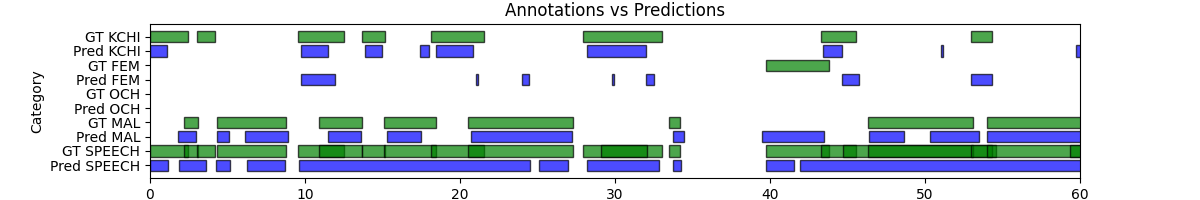
\includegraphics[width=6.67in]{images/vtc_performance_evaluation} 

}

\caption{VTC Predictions compared to Ground Truth Annotations}\label{fig:vtc-evaluations}
\end{figure}

\section{General Discussion}\label{general-discussion}

We present the ChildLens dataset, a unique egocentric video-audio dataset that documents children's everyday experiences, spanning a wide age range of 3 to 5 years. This dataset is particularly distinctive due to its diversity in terms of the number of children it includes and the variety of activity labels it covers. By focusing on both visual and auditory data, the ChildLens dataset provides comprehensive annotations for a broad spectrum of key activities, offering rich insights into children's social and behavioral interactions in naturalistic settings. This makes it a valuable resource for studying developmental processes in children, with a focus on their cognitive, emotional, and social growth.

In comparison to other freely available datasets, the ChildLens dataset stands out due to its broad age span and diverse set of activity labels. Most other datasets focus either on toddlers, are limited to dyadic interactions or were recorded in lab settings, with all of them lacking a comprehensive range of activity labels. Furthermore, most of these datasets either capture only audio or video, missing the multimodal aspect crucial for understanding children's everyday experiences. In contrast, ChildLens includes naturalistic recordings from children's home environments, over an extended period, and features a variety of activity types. The dataset also captures whether children are engaged in activities alone or with others and provides detailed demographic information about all individuals involved. This comprehensive approach enables a deeper and more holistic understanding of children's interactions and developmental trajectories.

The usefulness of the ChildLens dataset is demonstrated by its successful application to well-established models. For example, the pretrained Voice-Type Classifier for audio transcription achieves performance comparable to previous datasets, while the Boundary-Matching Network (BMN) produces robust results for activity localization, consistent with its performance on other datasets. These results indicate that the ChildLens dataset's annotations align well with model predictions, highlighting its quality and potential for multimodal research. Moreover, the successful application of these models demonstrates how the dataset can support and automate the analysis of children's everyday activities.

Expanding the potential for multi-method approaches, activity localization could be further enhanced by incorporating object identification, allowing for better tracking of the objects children interact with during daily routines, as demonstrated in adult-focused studies (Kazakos, Huh, Nagrani, Zisserman, \& Damen, 2021). Research by Bambach et al. (Bambach, Lee, Crandall, \& Yu, 2015) also emphasizes the importance of hand detection in egocentric video for activity recognition. Their work on using Convolutional Neural Networks for hand segmentation highlights how such techniques can differentiate activities, offering a deeper understanding of children's interactions and behaviors.

The integration of visual and auditory data in the ChildLens dataset enables a more detailed and comprehensive understanding of children's daily experiences. Complex activities such as pretend play and reading a book, which require both audio and video for accurate detection, exemplify the strength of this multimodal approach. While previous studies, such as those analyzing disfluencies in children's speech during computer game play (Yildirim \& Narayanan, 2009), have demonstrated that combining visual and auditory information can improve performance, few studies have explored this in the context of children's naturalistic activities. With ChildLens, the combination of naturalistic data and multimodal analysis creates new opportunities for in-depth insights into children's cognitive, emotional, and social development, particularly for activities best captured through both modalities.

Despite its strengths, one limitation of the ChildLens dataset is the class imbalance, especially in underrepresented activity classes, which could affect model training and evaluation. More frequent activities, such as ``child talking'' (7447 instances, 649 minutes) and ``playing with object'' (317 instances, 1371 minutes), dominate the dataset, whereas less common activities like ``dancing'' (2 instances, 0.57 minutes) and ``making music'' (2 instances, 2.13 minutes) are scarcely represented. Similarly, activities like ``pretend play'' (59 instances, 158.84 minutes) and ``reading a book'' (81 instances, 328.70 minutes) appear less frequently. This imbalance may lead to skewed model performance, making it harder to accurately classify rare activities. Possible solutions to this challenge could involve merging rare activity classes into broader categories or excluding them from model training, though these approaches may reduce the dataset's diversity. Other methods, such as resampling or augmentation, could help balance the dataset and improve model performance (Alani, Cosma, \& Taherkhani, 2020; Spelmen \& Porkodi, 2018).

In addition to class imbalance, another potential limitation is the sampling bias. Since the recordings are largely influenced by parental decisions about when and how often activities are captured, certain activities or settings may be overrepresented or underrepresented based on these preferences. Furthermore, the dataset primarily focuses on families from a mid-sized German city, limiting its geographic and cultural diversity. Expanding the dataset to include a broader range of families from different regions and cultures would enhance its generalizability and applicability to various research contexts.

The study of children's everyday experiences is crucial for understanding their cognitive, emotional, and social development. These daily interactions provide important insights into how children learn, grow, and engage with their environment. The ChildLens dataset makes a valuable contribution to this field by offering a rich multimodal resource that captures the complexities of children's lives in naturalistic settings. With its comprehensive annotations and potential to automate the analysis of children's activities, the dataset enables researchers to gain deeper and more detailed insights into children's development. By making such analyses more efficient and accessible, the ChildLens dataset creates new opportunities for understanding the complexities of early childhood development and provides a foundation for future research in this area.

\newpage

\section{References}\label{references}

\begingroup
\setlength{\parindent}{-0.5in}
\setlength{\leftskip}{0.5in}

\phantomsection\label{refs}
\begin{CSLReferences}{1}{0}
\bibitem[\citeproctext]{ref-alaniClassifyingImbalancedMultimodal2020}
Alani, A. A., Cosma, G., \& Taherkhani, A. (2020). Classifying {Imbalanced Multi-modal Sensor Data} for {Human Activity Recognition} in a {Smart Home} using {Deep Learning}. \emph{2020 {International Joint Conference} on {Neural Networks} ({IJCNN})}, 1--8. Glasgow, United Kingdom: IEEE. \url{https://doi.org/10.1109/IJCNN48605.2020.9207697}

\bibitem[\citeproctext]{ref-baevskiWav2vec20Framework2020}
Baevski, A., Zhou, H., Mohamed, A., \& Auli, M. (2020). Wav2vec 2.0: {A Framework} for {Self-Supervised Learning} of {Speech Representations}. \url{https://doi.org/10.48550/ARXIV.2006.11477}

\bibitem[\citeproctext]{ref-bambachLendingHandDetecting2015}
Bambach, S., Lee, S., Crandall, D. J., \& Yu, C. (2015). Lending {A Hand}: {Detecting Hands} and {Recognizing Activities} in {Complex Egocentric Interactions}. \emph{2015 {IEEE International Conference} on {Computer Vision} ({ICCV})}, 1949--1957. Santiago, Chile: IEEE. \url{https://doi.org/10.1109/ICCV.2015.226}

\bibitem[\citeproctext]{ref-bergelsonEverydayLanguageInput2023}
Bergelson, E., Soderstrom, M., Schwarz, I.-C., Rowland, C. F., Ramírez-Esparza, N., R. Hamrick, L., \ldots{} Cristia, A. (2023). Everyday language input and production in 1,001 children from six continents. \emph{Proceedings of the National Academy of Sciences}, \emph{120}(52), e2300671120. \url{https://doi.org/10.1073/pnas.2300671120}

\bibitem[\citeproctext]{ref-bredinPyannoteaudio21Speaker2023}
Bredin, H. (2023). Pyannote.audio 2.1 speaker diarization pipeline: Principle, benchmark, and recipe. \emph{{INTERSPEECH} 2023}, 1983--1987. ISCA. \url{https://doi.org/10.21437/Interspeech.2023-105}

\bibitem[\citeproctext]{ref-caoOpenPoseRealtimeMultiPerson2018}
Cao, Z., Hidalgo, G., Simon, T., Wei, S.-E., \& Sheikh, Y. (2018). {OpenPose}: {Realtime Multi-Person 2D Pose Estimation} using {Part Affinity Fields}. \url{https://doi.org/10.48550/ARXIV.1812.08008}

\bibitem[\citeproctext]{ref-carpendaleWhatMakesUs2020}
Carpendale, J., \& Lewis, C. (2020). \emph{What {Makes Us Human}: {How Minds Develop} through {Social Interactions}} (1st ed.). Routledge. \url{https://doi.org/10.4324/9781003125105}

\bibitem[\citeproctext]{ref-carreiraQuoVadisAction2017}
Carreira, J., \& Zisserman, A. (2017). Quo {Vadis}, {Action Recognition}? {A New Model} and the {Kinetics Dataset}. \url{https://doi.org/10.48550/ARXIV.1705.07750}

\bibitem[\citeproctext]{ref-chenDyadicAffectParentChild2023}
Chen, H., Alghowinem, S., Jang, S. J., Breazeal, C., \& Park, H. W. (2023). Dyadic {Affect} in {Parent-Child Multimodal Interaction}: {Introducing} the {DAMI-P2C Dataset} and its {Preliminary Analysis}. \emph{IEEE Transactions on Affective Computing}, \emph{14}(4), 3345--3361. \url{https://doi.org/10.1109/TAFFC.2022.3178689}

\bibitem[\citeproctext]{ref-mmaction2contributorsOpenMMLabsNextGeneration2020}
Contributors, M. (2020). \emph{{OpenMMLab}'s {Next Generation Video Understanding Toolbox} and {Benchmark}}. Retrieved from \url{urlhttps://github.com/open-mmlab/mmaction2}

\bibitem[\citeproctext]{ref-debarbaroTenLessonsInfants2022}
De Barbaro, K., \& Fausey, C. M. (2022). Ten {Lessons About Infants}' {Everyday Experiences}. \emph{Current Directions in Psychological Science}, \emph{31}(1), 28--33. \url{https://doi.org/10.1177/09637214211059536}

\bibitem[\citeproctext]{ref-donnellyLongitudinalRelationshipConversational2021}
Donnelly, S., \& Kidd, E. (2021). The {Longitudinal Relationship Between Conversational Turn}‐{Taking} and {Vocabulary Growth} in {Early Language Development}. \emph{Child Development}, \emph{92}(2), 609--625. \url{https://doi.org/10.1111/cdev.13511}

\bibitem[\citeproctext]{ref-fraileUpStoryUppsalaStorytelling2024}
Fraile, M., Calvo-Barajas, N., Apeiron, A. S., Varni, G., Lindblad, J., Sladoje, N., \& Castellano, G. (2024). {UpStory}: The {Uppsala Storytelling} dataset. \url{https://doi.org/10.48550/ARXIV.2407.04352}

\bibitem[\citeproctext]{ref-heyesCognitiveGadgetsCultural2018}
Heyes, C. M. (2018). \emph{Cognitive gadgets: The cultural evolution of thinking}. Cambridge (Mass.): Harvard University press.

\bibitem[\citeproctext]{ref-kazakosLittleHelpMy2021}
Kazakos, E., Huh, J., Nagrani, A., Zisserman, A., \& Damen, D. (2021). With a {Little Help} from my {Temporal Context}: {Multimodal Egocentric Action Recognition}. \url{https://doi.org/10.48550/ARXIV.2111.01024}

\bibitem[\citeproctext]{ref-lavechinOpensourceVoiceType2020}
Lavechin, M., Bousbib, R., Bredin, H., Dupoux, E., \& Cristia, A. (2020). An open-source voice type classifier for child-centered daylong recordings. \url{https://doi.org/10.48550/ARXIV.2005.12656}

\bibitem[\citeproctext]{ref-linBMNBoundaryMatchingNetwork2019}
Lin, T., Liu, X., Li, X., Ding, E., \& Wen, S. (2019). {BMN}: {Boundary-Matching Network} for {Temporal Action Proposal Generation}. \url{https://doi.org/10.48550/ARXIV.1907.09702}

\bibitem[\citeproctext]{ref-longBabyViewDatasetHighresolution2024}
Long, B., Xiang, V., Stojanov, S., Sparks, R. Z., Yin, Z., Keene, G. E., \ldots{} Frank, M. C. (2024, June 14). The {BabyView} dataset: {High-resolution} egocentric videos of infants' and young children's everyday experiences. \url{https://doi.org/10.48550/arXiv.2406.10447}

\bibitem[\citeproctext]{ref-piagetPartCognitiveDevelopment1964}
Piaget, J. (1964). Part {I}: {Cognitive} development in children: {Piaget} development and learning. \emph{Journal of Research in Science Teaching}, \emph{2}(3), 176--186. \url{https://doi.org/10.1002/tea.3660020306}

\bibitem[\citeproctext]{ref-plaquetPowersetMulticlassCross2023}
Plaquet, A., \& Bredin, H. (2023). Powerset multi-class cross entropy loss for neural speaker diarization. \emph{{INTERSPEECH} 2023}, 3222--3226. ISCA. \url{https://doi.org/10.21437/Interspeech.2023-205}

\bibitem[\citeproctext]{ref-redmonYouOnlyLook2015}
Redmon, J., Divvala, S., Girshick, R., \& Farhadi, A. (2015). You {Only Look Once}: {Unified}, {Real-Time Object Detection}. \url{https://doi.org/10.48550/ARXIV.1506.02640}

\bibitem[\citeproctext]{ref-rehgDecodingChildrensSocial2013}
Rehg, J. M., Abowd, G. D., Rozga, A., Romero, M., Clements, M. A., Sclaroff, S., \ldots{} Ye, Z. (2013). Decoding {Children}'s {Social Behavior}. \emph{2013 {IEEE Conference} on {Computer Vision} and {Pattern Recognition}}, 3414--3421. Portland, OR, USA: IEEE. \url{https://doi.org/10.1109/CVPR.2013.438}

\bibitem[\citeproctext]{ref-rogoffImportanceUnderstandingChildrens2018}
Rogoff, B., Dahl, A., \& Callanan, M. (2018). The importance of understanding children's lived experience. \emph{Developmental Review}, \emph{50}, 5--15. \url{https://doi.org/10.1016/j.dr.2018.05.006}

\bibitem[\citeproctext]{ref-roweDifferencesEarlyGesture2009}
Rowe, M. L., \& Goldin-Meadow, S. (2009). Differences in {Early Gesture Explain SES Disparities} in {Child Vocabulary Size} at {School Entry}. \emph{Science}, \emph{323}(5916), 951--953. \url{https://doi.org/10.1126/science.1167025}

\bibitem[\citeproctext]{ref-royPredictingBirthSpoken2015}
Roy, B. C., Frank, M. C., DeCamp, P., Miller, M., \& Roy, D. (2015). Predicting the birth of a spoken word. \emph{Proceedings of the National Academy of Sciences}, \emph{112}(41), 12663--12668. \url{https://doi.org/10.1073/pnas.1419773112}

\bibitem[\citeproctext]{ref-ruffmanExposureBehavioralRegularities2023}
Ruffman, T., Chen, L., Lorimer, B., Vanier, S., Edgar, K., Scarf, D., \& Taumoepeau, M. (2023). Exposure to behavioral regularities in everyday life predicts infants' acquisition of mental state vocabulary. \emph{Developmental Science}, \emph{26}(4), e13343. \url{https://doi.org/10.1111/desc.13343}

\bibitem[\citeproctext]{ref-russakovskyImageNetLargeScale2014}
Russakovsky, O., Deng, J., Su, H., Krause, J., Satheesh, S., Ma, S., \ldots{} Fei-Fei, L. (2014). {ImageNet Large Scale Visual Recognition Challenge}. \url{https://doi.org/10.48550/ARXIV.1409.0575}

\bibitem[\citeproctext]{ref-smithDevelopingInfantCreates2018}
Smith, L. B., Jayaraman, S., Clerkin, E., \& Yu, C. (2018). The {Developing Infant Creates} a {Curriculum} for {Statistical Learning}. \emph{Trends in Cognitive Sciences}, \emph{22}(4), 325--336. \url{https://doi.org/10.1016/j.tics.2018.02.004}

\bibitem[\citeproctext]{ref-spanglerToddlersEverydayExperiences1989}
Spangler, G. (1989). Toddlers' {Everyday Experiences} as {Related} to {Preceding Mental} and {Emotional Disposition} and {Their Relationship} to {Subsequent Mental} and {Motivational Development}: {A Short-Term Longitudinal Study}. \emph{International Journal of Behavioral Development}, \emph{12}(3), 285--303. \url{https://doi.org/10.1177/016502548901200301}

\bibitem[\citeproctext]{ref-spelmenReviewHandlingImbalanced2018}
Spelmen, V. S., \& Porkodi, R. (2018). A {Review} on {Handling Imbalanced Data}. \emph{2018 {International Conference} on {Current Trends} Towards {Converging Technologies} ({ICCTCT})}, 1--11. Coimbatore: IEEE. \url{https://doi.org/10.1109/ICCTCT.2018.8551020}

\bibitem[\citeproctext]{ref-sullivanSAYCamLargeLongitudinal2021}
Sullivan, J., Mei, M., Perfors, A., Wojcik, E., \& Frank, M. C. (2021). {SAYCam}: {A Large}, {Longitudinal Audiovisual Dataset Recorded From} the {Infant}'s {Perspective}. \emph{Open Mind}, \emph{5}, 20--29. \url{https://doi.org/10.1162/opmi_a_00039}

\bibitem[\citeproctext]{ref-tomaselloCulturalOriginsHuman2009}
Tomasello, M. (2009). \emph{Cultural {Origins} of {Human Cognition}}. Cambridge: Harvard University Press.

\bibitem[\citeproctext]{ref-vygotskyMindSocietyDevelopment1978}
Vygotsky, L. S. (1978). \emph{Mind in {Society}: {The Development} of {Higher Psychological Processes}}. Cambridge, MA: Harvard University Press.

\bibitem[\citeproctext]{ref-yildirimAutomaticDetectionDisfluency2009}
Yildirim, S., \& Narayanan, S. (2009). Automatic {Detection} of {Disfluency Boundaries} in {Spontaneous Speech} of {Children Using Audio}\&\#x2013;{Visual Information}. \emph{IEEE Transactions on Audio, Speech, and Language Processing}, \emph{17}(1), 2--12. \url{https://doi.org/10.1109/TASL.2008.2006728}

\end{CSLReferences}

\endgroup

\newpage

\section{Appendix}\label{appendix}

\subsection{List of ChildLens Activity Classes}\label{list-of-childlens-activity-classes}

The dataset contains the following list of activities.

\begin{enumerate}
\def\labelenumi{\arabic{enumi}.}
\tightlist
\item
  \textbf{playing with object}: The child is playing with an object, such as a toy or a ball.
\item
  \textbf{playing without object}: The child is playing without an object, such as playing hide and seek or catch.
\item
  \textbf{pretend play}: The child is engaged in imaginative play, such as pretending to be a doctor or a firefighter.
\item
  \textbf{watching something}: The child is watching a movie, TV show, or video on either a screen or a device.
\item
  \textbf{reading book}: The child is reading a book or looking at pictures in a book.
\item
  \textbf{child talking}: The child is talking to themselves or to someone else.
\item
  \textbf{other person talking}: Another person is talking to the child.
\item
  \textbf{overheard speech}: Conversations that the child can hear but is not directly involved in.
\item
  \textbf{drawing}: The child is drawing or coloring a picture.
\item
  \textbf{crafting things}: The child is engaged in a craft activity, such as making a bracelet or decoration.
\item
  \textbf{singing / humming}: The child is singing or humming a song or a melody.
\item
  \textbf{making music}: The child is playing a musical instrument or making music in another way.
\item
  \textbf{dancing}: The child is dancing to music or moving to a rhythm.
\item
  \textbf{listening to music / audiobook}: The child is listening to music or an audiobook.
\end{enumerate}

\subsection{List of ChildLens Location Classes}\label{list-of-childlens-location-classes}

\begin{enumerate}
\def\labelenumi{\arabic{enumi}.}
\tightlist
\item
  livingroom
\item
  playroom
\item
  bathroom
\item
  hallway
\item
  other
\end{enumerate}

\subsection{Activity Class Statistics}\label{activity-class-statistics}

\begin{table}[tbp]

\begin{center}
\begin{threeparttable}

\caption{\label{tab:activity-classes-statistics}Number of video instances and the total duration (in minutes).}

\begin{tabular}{llll}
\toprule
Category & \multicolumn{1}{c}{Activity Class} & \multicolumn{1}{c}{Instance Count} & \multicolumn{1}{c}{Total Duration (min)}\\
\midrule
Audio & Child talking & 7447 & 649.10\\
 & Other person talking & 6113 & 455.29\\
 & Overheard Speech & 1898 & 299.44\\
 & Singing/Humming & 277 & 82.00\\
 & Listening to music/audiobook & 68 & 222.14\\
Video & Watching something & 2 & 5.09\\
 & Drawing & 62 & 374.91\\
 & Crafting things & 26 & 109.14\\
 & Dancing & 2 & 0.57\\
Multimodal & Playing with object & 317 & 1371.06\\
 & Playing without object & 25 & 28.87\\
 & Pretend play & 59 & 158.84\\
 & Reading a book & 81 & 328.70\\
 & Making music & 3 & 2.13\\
\bottomrule
\end{tabular}

\end{threeparttable}
\end{center}

\end{table}


\end{document}
